\documentclass{standalone}
\usepackage{tikz}
\begin{document}
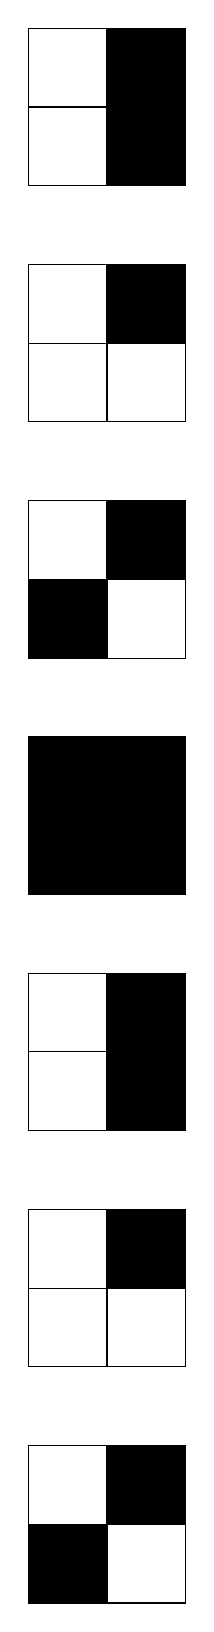
\begin{tikzpicture}
\begin{scope}[shift={(0,0)}]
\draw (0,0) grid (2,-2);
\draw (0,0) rectangle (1,-1);
\draw[fill] (1,0) rectangle (2,-1);
\draw (0,-1) rectangle (1,-2);
\draw[fill] (1,-1) rectangle (2,-2);
\end{scope}
\begin{scope}[shift={(0,-3)}]
\draw (0,0) grid (2,-2);
\draw (0,0) rectangle (1,-1);
\draw[fill] (1,0) rectangle (2,-1);
\draw (0,-1) rectangle (1,-2);
\draw (1,-1) rectangle (2,-2);
\end{scope}
\begin{scope}[shift={(0,-6)}]
\draw (0,0) grid (2,-2);
\draw (0,0) rectangle (1,-1);
\draw[fill] (1,0) rectangle (2,-1);
\draw[fill] (0,-1) rectangle (1,-2);
\draw (1,-1) rectangle (2,-2);
\end{scope}
\begin{scope}[shift={(0,-9)}]
\draw (0,0) grid (2,-2);
\draw[fill] (0,0) rectangle (1,-1);
\draw[fill] (1,0) rectangle (2,-1);
\draw[fill] (0,-1) rectangle (1,-2);
\draw[fill] (1,-1) rectangle (2,-2);
\end{scope}
\begin{scope}[shift={(0,-12)}]
\draw (0,0) grid (2,-2);
\draw (0,0) rectangle (1,-1);
\draw[fill] (1,0) rectangle (2,-1);
\draw (0,-1) rectangle (1,-2);
\draw[fill] (1,-1) rectangle (2,-2);
\end{scope}
\begin{scope}[shift={(0,-15)}]
\draw (0,0) grid (2,-2);
\draw (0,0) rectangle (1,-1);
\draw[fill] (1,0) rectangle (2,-1);
\draw (0,-1) rectangle (1,-2);
\draw (1,-1) rectangle (2,-2);
\end{scope}
\begin{scope}[shift={(0,-18)}]
\draw (0,0) grid (2,-2);
\draw (0,0) rectangle (1,-1);
\draw[fill] (1,0) rectangle (2,-1);
\draw[fill] (0,-1) rectangle (1,-2);
\draw (1,-1) rectangle (2,-2);
\end{scope}
\end{tikzpicture}
\end{document}
